% Options for packages loaded elsewhere
\PassOptionsToPackage{unicode}{hyperref}
\PassOptionsToPackage{hyphens}{url}
\PassOptionsToPackage{dvipsnames,svgnames,x11names}{xcolor}
\documentclass[
  10pt,
  fontset=fandol]{ctexart}
\usepackage{xcolor}
\usepackage[margin=16mm]{geometry}
\usepackage{amsmath,amssymb}
\setcounter{secnumdepth}{-\maxdimen} % remove section numbering
\usepackage{iftex}
\ifPDFTeX
  \usepackage[T1]{fontenc}
  \usepackage[utf8]{inputenc}
  \usepackage{textcomp} % provide euro and other symbols
\else % if luatex or xetex
  \usepackage{unicode-math} % this also loads fontspec
  \defaultfontfeatures{Scale=MatchLowercase}
  \defaultfontfeatures[\rmfamily]{Ligatures=TeX,Scale=1}
\fi
\usepackage{lmodern}
\ifPDFTeX\else
  % xetex/luatex font selection
\fi
% Use upquote if available, for straight quotes in verbatim environments
\IfFileExists{upquote.sty}{\usepackage{upquote}}{}
\IfFileExists{microtype.sty}{% use microtype if available
  \usepackage[]{microtype}
  \UseMicrotypeSet[protrusion]{basicmath} % disable protrusion for tt fonts
}{}
\makeatletter
\@ifundefined{KOMAClassName}{% if non-KOMA class
  \IfFileExists{parskip.sty}{%
    \usepackage{parskip}
  }{% else
    \setlength{\parindent}{0pt}
    \setlength{\parskip}{6pt plus 2pt minus 1pt}}
}{% if KOMA class
  \KOMAoptions{parskip=half}}
\makeatother
\usepackage{longtable,booktabs,array}
\newcounter{none} % for unnumbered tables
\usepackage{calc} % for calculating minipage widths
% Correct order of tables after \paragraph or \subparagraph
\usepackage{etoolbox}
\makeatletter
\patchcmd\longtable{\par}{\if@noskipsec\mbox{}\fi\par}{}{}
\makeatother
% Allow footnotes in longtable head/foot
\IfFileExists{footnotehyper.sty}{\usepackage{footnotehyper}}{\usepackage{footnote}}
\makesavenoteenv{longtable}
\usepackage{graphicx}
\makeatletter
\newsavebox\pandoc@box
\newcommand*\pandocbounded[1]{% scales image to fit in text height/width
  \sbox\pandoc@box{#1}%
  \Gscale@div\@tempa{\textheight}{\dimexpr\ht\pandoc@box+\dp\pandoc@box\relax}%
  \Gscale@div\@tempb{\linewidth}{\wd\pandoc@box}%
  \ifdim\@tempb\p@<\@tempa\p@\let\@tempa\@tempb\fi% select the smaller of both
  \ifdim\@tempa\p@<\p@\scalebox{\@tempa}{\usebox\pandoc@box}%
  \else\usebox{\pandoc@box}%
  \fi%
}
% Set default figure placement to htbp
\def\fps@figure{htbp}
\makeatother
\setlength{\emergencystretch}{3em} % prevent overfull lines
\providecommand{\tightlist}{%
  \setlength{\itemsep}{0pt}\setlength{\parskip}{0pt}}
\usepackage{amsmath,amssymb,mathtools,needspace}
\xeCJKDeclareCharClass{CJK}{"2032,"0400->"04FF,"2160->"216B,"2460->"2473,"25A0,"25C7,"25CB,"25CF}
\IfFontExistsTF{Arial Unicode MS}{\xeCJKsetup{AutoFallBack=true}\setCJKfallbackfamilyfont{\CJKrmdefault}{Arial Unicode MS}}{}
\setcounter{secnumdepth}{0}
\setlength{\emergencystretch}{2em}
\allowdisplaybreaks
\usepackage{bookmark}
\IfFileExists{xurl.sty}{\usepackage{xurl}}{} % add URL line breaks if available
\urlstyle{same}
\hypersetup{
  pdftitle={差分与等距节点插值公式},
  colorlinks=true,
  linkcolor={Maroon},
  filecolor={Maroon},
  citecolor={Blue},
  urlcolor={Blue},
  pdfcreator={LaTeX via pandoc}}

\title{差分与等距节点插值公式}
\author{}
\date{}

\begin{document}
\maketitle

\subsection{2.5 差分与等距节点插值公式}\label{ux5deeux5206ux4e0eux7b49ux8dddux8282ux70b9ux63d2ux503cux516cux5f0f}

上面讨论了节点任意分布的插值公式，但实际应用时经常遇到等距节点的情形，这时插值公式可以进一步简化，计算也简单得多。为了得到等距节点的插值公式，下面先介绍差分的概念。

\subsubsection{2.5.1 差分及其性质}\label{ux5deeux5206ux53caux5176ux6027ux8d28}

设函数 \(y=f(x)\) 在等距节点 \(x_k=x_0+kh\;(k=0,1,\cdots,n)\) 上的值 \(f_k=f(x_k)\) 为已知，这里 \(h\) 为常数，称为\textbf{步长}。

\textbf{定义 2.4} 偏差

\[
\Delta f_k=f_{k+1}-f_k,
\tag{2.5.1}
\]

\[
\nabla f_k=f_k-f_{k-1},
\tag{2.5.2}
\]

\[
\delta f_k=f(x_k+h/2)-f(x_k-h/2)=f_{k+\frac12}-f_{k-\frac12}
\tag{2.5.3}
\]

分别称为 \(f(x)\) 在 \(x_k\) 处以 \(h\) 为步长的\textbf{向前差分}、\textbf{向后差分}及\textbf{中心差分}。符号 \(\Delta,\nabla,\delta\) 分别称为\textbf{向前差分算子}、\textbf{向后差分算子}及\textbf{中心差分算子}。

利用一阶差分可定义二阶差分为

\[
\Delta^2 f_k=\Delta f_{k+1}-\Delta f_k=f_{k+2}-2f_{k+1}+f_k.
\]

一般地，可定义 \(m\) 阶差分为

\[
\Delta^m f_k=\Delta^{m-1}f_{k+1}-\Delta^{m-1}f_k,\qquad
\nabla^m f_k=\nabla^{m-1}f_k-\nabla^{m-1}f_{k-1}.
\]

因中心差分 \(\delta f_k\) 用到 \(f_{k+\frac12}\) 及 \(f_{k-\frac12}\) 这两个值，实际上不是函数表上的值。如果用函数表上的值，一阶中心差分应写成

\[
\delta f_{k+\frac12}=f_{k+1}-f_k,\qquad
\delta f_{k-\frac12}=f_k-f_{k-1};
\]

二阶中心差分为 \(\delta^2 f_k=\delta f_{k+\frac12}-\delta f_{k-\frac12}\)；等等。

除了已引入的差分算子外，常用算子符号还有\textbf{不变算子 \(\mathrm{I}\)} 及\textbf{移位算子 \(\mathrm{E}\)}，定义如下：

\[
\mathrm{I}f_k=f_k,\qquad\mathrm{E}f_k=f_{k+1},
\]

于是，由 \(\Delta f_k=f_{k+1}-f_k=\mathrm{E}f_k-\mathrm{I}f_k=(\mathrm{E}-\mathrm{I})f_k\)，可得 \(\Delta=\mathrm{E}-\mathrm{I}\)。

同理，可得

\[
\nabla=\mathrm{I}-\mathrm{E}^{-1},\qquad
\delta=\mathrm{E}^{\frac12}-\mathrm{E}^{-\frac12}.
\]

由差分定义并应用算子符号运算可得下列基本性质。

\textbf{性质 1} 各阶差分均可用函数值表示。例如

\subsubsection{校注（agent 补充）：例 2.3 的误差估计范围}\label{ux6821ux6ce8agent-ux8865ux5145ux4f8b-2.3-ux7684ux8befux5deeux4f30ux8ba1ux8303ux56f4}

页首 \(3.63\times10^{-9}\) 使用原表 2.5 的五阶差商 \(-0.00012\) 及乘积 \(\omega_5(0.596)\) 得到，原文已使用近似号。原表高阶差商的舍入敏感性见 PDF 38 校注 CH02A-S03；仅凭给定的有限节点表值，不能对任意与这些节点相符的函数证明这一截断误差上界，节点数据的舍入误差也未计入。以上是 agent 的适用范围说明，原书结论仍在正文保留。

\subsubsection{校注（agent 补充）：CH02A-S04，例 2.3 的函数值结果}\label{ux6821ux6ce8agent-ux8865ux5145ch02a-s04ux4f8b-2.3-ux7684ux51fdux6570ux503cux7ed3ux679c}

原书本页实际印为 \(N_4(0.596)=0.63195\)，本转录保留该数。按 PDF 38 原印的四次多项式逐项代入 \(x=0.596\)，得到

\[
N_4(0.596)=0.63191751982370304,
\]

保留五位小数为 \(0.63192\)，与原书的 \(0.63195\) 不符。这一差异并非末位舍入造成，属于原书该计算结果的数值错误。

\href{../../source-images/pdf-040.jpeg}{原页：书页 27／PDF 40}

\begin{quote}
页首承接 PDF 39 的性质 1。
\end{quote}

\[
\Delta^n f_k=(\mathrm{E}-\mathrm{I})^n f_k
=\sum_{j=0}^{n}(-1)^j\binom{n}{j}\mathrm{E}^{n-j}f_k
=\sum_{j=0}^{n}(-1)^j\binom{n}{j}f_{n+k-j},
\tag{2.5.4}
\]

\[
\nabla^n f_k=(\mathrm{I}-\mathrm{E}^{-1})^n f_k
=\sum_{j=0}^{n}(-1)^{n-j}\binom{n}{j}\mathrm{E}^{j-n}f_k
=\sum_{j=0}^{n}(-1)^{n-j}\binom{n}{j}f_{k+j-n},
\tag{2.5.5}
\]

其中 \(\displaystyle\binom{n}{j}=\frac{n(n-1)\cdots(n-j+1)}{j!}\) 为二项式展开系数。

\textbf{性质 2} 可用各阶差分表示函数值，例如，可用向前差分表示 \(f_{n+k}\)，即

\[
f_{n+k}=\mathrm{E}^n f_k=(\mathrm{I}+\Delta)^n f_k=\sum_{j=0}^{n}\binom{n}{j}\Delta^j f_k.
\tag{2.5.6}
\]

\textbf{性质 3} 差商与差分有以下关系，例如，对于向前差分，由定义

\[
f[x_k,x_{k+1}]=\frac{f_{k+1}-f_k}{x_{k+1}-x_k}=\frac{\Delta f_k}{h},
\]

\[
f[x_k,x_{k+1},x_{k+2}]=\frac{f[x_{k+1},x_{k+2}]-f[x_k,x_{k+1}]}{x_{k+2}-x_k}=\frac{1}{2h^2}\Delta^2 f_k,
\]

一般地有

\[
f[x_k,x_{k+1},\cdots,x_{k+m}]=\frac{1}{m!}\frac{1}{h^m}\Delta^m f_k\qquad(m=1,2,\cdots,n).
\tag{2.5.7}
\]

同理，对于向后差分，有

\[
f[x_k,x_{k-1},\cdots,x_{k-m}]=\frac{1}{m!}\frac{1}{h^m}\nabla^m f_k.
\tag{2.5.8}
\]

利用式（2.5.7）及式（2.4.5）又可得到

\[
\Delta^n f_k=h^n f^{(n)}(\xi),
\tag{2.5.9}
\]

其中 \(\xi\in(x_k,x_{k+n})\)，这是差分与导数的关系。差分的其他性质可参看习题 10～12。

计算差分可列差分表，表 2.6 是向前差分表。

\textbf{表 2.6}

{\def\LTcaptype{none} % do not increment counter
\begin{longtable}[]{@{}
  >{\raggedright\arraybackslash}p{(\linewidth - 8\tabcolsep) * \real{0.2000}}
  >{\raggedright\arraybackslash}p{(\linewidth - 8\tabcolsep) * \real{0.2000}}
  >{\raggedright\arraybackslash}p{(\linewidth - 8\tabcolsep) * \real{0.2000}}
  >{\raggedright\arraybackslash}p{(\linewidth - 8\tabcolsep) * \real{0.2000}}
  >{\raggedright\arraybackslash}p{(\linewidth - 8\tabcolsep) * \real{0.2000}}@{}}
\toprule\noalign{}
\begin{minipage}[b]{\linewidth}\raggedright
\(x_k\)
\end{minipage} & \begin{minipage}[b]{\linewidth}\raggedright
\(\Delta\)
\end{minipage} & \begin{minipage}[b]{\linewidth}\raggedright
\(\Delta^2\)
\end{minipage} & \begin{minipage}[b]{\linewidth}\raggedright
\(\Delta^3\)
\end{minipage} & \begin{minipage}[b]{\linewidth}\raggedright
\(\Delta^4\)
\end{minipage} \\
\midrule\noalign{}
\endhead
\bottomrule\noalign{}
\endlastfoot
\(f_0\) & \(\Delta f_0\) & \(\Delta^2 f_0\) & \(\Delta^3 f_0\) & \(\Delta^4 f_0\) \\
\(f_1\) & \(\Delta f_1\) & \(\Delta^2 f_1\) & \(\Delta^3 f_1\) & \(\vdots\) \\
\(f_2\) & \(\Delta f_2\) & \(\Delta^2 f_2\) & \(\vdots\) & \\
\(f_3\) & \(\Delta f_3\) & \(\vdots\) & & \\
\(f_4\) & \(\vdots\) & & & \\
\(\vdots\) & & & & \\
\end{longtable}
}

\subsubsection{校注（agent 补充）：CH02A-S02，表 2.6 的首列表头}\label{ux6821ux6ce8agent-ux8865ux5145ch02a-s02ux8868-2.6-ux7684ux9996ux5217ux8868ux5934}

原书表 2.6 首列表头实际印为 \(x_k\)，而其内容为 \(f_0,f_1,\cdots\)，本转录均按原图保留。依各阶向前差分的意义，该列存放函数值，表头应理解为 \(f_k\)；这是原书表头与内容不一致的问题。CH02A-S02 是本 lane 的临时校注编号。

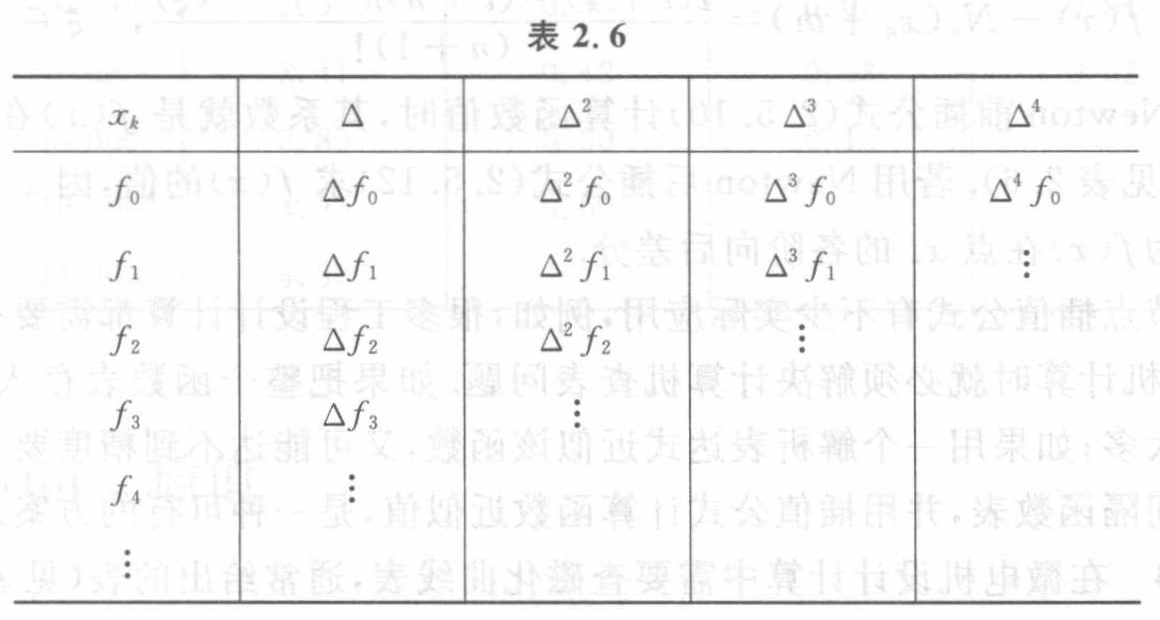
\includegraphics[width=0.85\linewidth,height=\textheight,keepaspectratio,alt={表 2.6 原图裁切}]{../assets/ch02a/pdf-040-table-2.6.png}

\href{../../source-images/pdf-041.jpeg}{原页：书页 28／PDF 41}

\subsubsection{2.5.2 等距节点插值公式}\label{ux7b49ux8dddux8282ux70b9ux63d2ux503cux516cux5f0f}

将 Newton 差商插值多项式（2.4.6）中各阶差商用相应差分代替，就可得到各种形式的等距节点插值公式。这里只推导常用的前插公式与后插公式。

如果节点 \(x_k=x_0+kh\;(k=0,1,\cdots,n)\)，要计算 \(x_0\) 附近点 \(x\) 的函数 \(f(x)\) 的值，可令 \(x=x_0+th\)，\(0\le t\le1\)，于是

\[
\omega_{k+1}(x)=\prod_{j=0}^{k}(x-x_j)=t(t-1)\cdots(t-k)h^{k+1}.
\]

将此式及式（2.5.7）代入式（2.4.6），得

\[
N_n(x_0+th)=f_0+t\Delta f_0+\frac{t(t-1)}{2!}\Delta^2 f_0+\cdots+\frac{t(t-1)\cdots(t-n+1)}{n!}\Delta^n f_0.
\tag{2.5.10}
\]

式（2.5.10）称为 \textbf{Newton 前插公式}，其余项由式（2.2.14）得

\[
R_n(x)=\frac{t(t-1)\cdots(t-n)}{(n+1)!}h^{n+1}f^{(n+1)}(\xi),\qquad\xi\in(x_0,x_n).
\tag{2.5.11}
\]

如果要求表示函数在 \(x_n\) 附近的值 \(f(x)\)，此时应用 Newton 插值公式（2.4.6），插值点应按 \(x_n,x_{n-1},\cdots,x_0\) 的次序排列，有

\[
\begin{aligned}
N_n(x)={}&f(x_n)+f[x_n,x_{n-1}](x-x_n)+f[x_n,x_{n-1},x_{n-2}](x-x_n)(x-x_{n-1})\\
&+\cdots+f[x_n,x_{n-1},\cdots,x_0](x-x_n)\cdots(x-x_1).
\end{aligned}
\]

作变换 \(x=x_n+th\;(-1\le t\le0)\)，并利用式（2.5.8），代入上式得

\[
\begin{aligned}
N_n(x_n+th)={}&f_n+t\nabla f_n+\frac{t(t+1)}{2!}\nabla^2 f_n+\cdots\\
&+\frac{t(t+1)\cdots(t+n-1)}{n!}\nabla^n f_n.
\end{aligned}
\tag{2.5.12}
\]

式（2.5.12）称为 \textbf{Newton 后插公式}，其余项

\[
R_n(x)=f(x)-N_n(x_n+th)=\frac{t(t+1)\cdots(t+n)h^{n+1}f^{(n+1)}(\xi)}{(n+1)!},\qquad\xi\in(x_0,x_n).
\]

利用 Newton 前插公式（2.5.10）计算函数值时，其系数就是 \(f(x)\) 在 \(x_0\) 的各阶向前差分（见表 2.6）。若用 Newton 后插公式（2.5.12）求 \(f(x)\) 的值，因 \(x\) 在 \(x_n\) 附近，则其系数为 \(f(x)\) 在点 \(x_n\) 的各阶向后差分。

等距节点插值公式有不少实际应用，例如，很多工程设计计算都需要查各种函数表，用计算机计算时就必须解决计算机查表问题。如果把整个函数表存入内存，往往占用单元太多；如果用一个解析表达式近似该函数，又可能达不到精度要求。因此，采用存放大间隔函数表，并用插值公式计算函数近似值，是一种可行的方案。

\textbf{例 2.4} 在微电机设计计算中需要查磁化曲线表，通常给出的表（见表 2.7）是磁密 \(B\) 每间隔 100 高斯磁路每厘米长所需安匝数 \(at\) 的值，下面要解决 \(B\) 从 \(4\,000\) 至

\begin{quote}
例 2.4 的区间上限及解答续 PDF 42。
\end{quote}

\href{../../source-images/pdf-042.jpeg}{原页：书页 29／PDF 42}

\begin{quote}
页首接 PDF 41 例 2.4 的区间；页末 2.6 首句续 PDF 43。
\end{quote}

\(11\,000\) 区间的查表问题。

\textbf{解} 为节省计算机存储单元，采用每 500 高斯存入一个 \(at\) 值。为了分析使用几阶插值公式合适，应先列出差分表。表 2.7 是以硅钢片的磁化曲线为例所造的差分表。

从差分表中看到三阶差分近似于 0，因此计算时只需用二阶差分，当 \(4\,000\le B\le10\,500\) 时用 Newton 前插公式，当 \(10\,500<B\le11\,000\) 时用 Newton 后插公式。例如，求 \(f(5\,200)\) 时取 \(B_0=5\,000\)，\(f_0=1.58\)，\(\Delta f_0=0.11\)，\(\Delta^2 f_0=0.01\)，\(h=500\)，\(B=5\,200\)，\(t=0.4\)，于是由式（2.5.10），取 \(n=2\)，得

\[
f(5\,200)\approx1.58+0.4\times0.11+\frac{0.4\times(-0.6)}{2}\times0.01\approx1.62.
\]

这个结果与直接查表得到的值相同，说明用此法在计算机上求 \(at\) 值是可行的。具体的查表程序作为练习由读者完成。

\textbf{表 2.7}

{\def\LTcaptype{none} % do not increment counter
\begin{longtable}[]{@{}
  >{\raggedleft\arraybackslash}p{(\linewidth - 10\tabcolsep) * \real{0.1667}}
  >{\raggedleft\arraybackslash}p{(\linewidth - 10\tabcolsep) * \real{0.1667}}
  >{\raggedleft\arraybackslash}p{(\linewidth - 10\tabcolsep) * \real{0.1667}}
  >{\raggedleft\arraybackslash}p{(\linewidth - 10\tabcolsep) * \real{0.1667}}
  >{\raggedleft\arraybackslash}p{(\linewidth - 10\tabcolsep) * \real{0.1667}}
  >{\raggedleft\arraybackslash}p{(\linewidth - 10\tabcolsep) * \real{0.1667}}@{}}
\toprule\noalign{}
\begin{minipage}[b]{\linewidth}\raggedleft
\(k\)
\end{minipage} & \begin{minipage}[b]{\linewidth}\raggedleft
\(B_k\)
\end{minipage} & \begin{minipage}[b]{\linewidth}\raggedleft
\(at_k=f(B_k)\)
\end{minipage} & \begin{minipage}[b]{\linewidth}\raggedleft
\(\Delta f_k\)
\end{minipage} & \begin{minipage}[b]{\linewidth}\raggedleft
\(\Delta^2 f_k\)
\end{minipage} & \begin{minipage}[b]{\linewidth}\raggedleft
\(\Delta^3 f_k\)
\end{minipage} \\
\midrule\noalign{}
\endhead
\bottomrule\noalign{}
\endlastfoot
\(0\) & \(4\,000\) & \(1.38\) & \(0.10\) & \(0\) & \(0.01\) \\
\(1\) & \(4\,500\) & \(1.48\) & \(0.10\) & \(0.01\) & \(0\) \\
\(2\) & \(5\,000\) & \(1.58\) & \(0.11\) & \(0.01\) & \(0\) \\
\(3\) & \(5\,500\) & \(1.69\) & \(0.12\) & \(0.01\) & \(0.02\) \\
\(4\) & \(6\,000\) & \(1.81\) & \(0.13\) & \(0.03\) & \(-0.01\) \\
\(5\) & \(6\,500\) & \(1.94\) & \(0.16\) & \(0.02\) & \(0.02\) \\
\(6\) & \(7\,000\) & \(2.10\) & \(0.18\) & \(0.04\) & \(0\) \\
\(7\) & \(7\,500\) & \(2.28\) & \(0.22\) & \(0.04\) & \(0\) \\
\(8\) & \(8\,000\) & \(2.50\) & \(0.26\) & \(0.04\) & \(0.01\) \\
\(9\) & \(8\,500\) & \(2.76\) & \(0.30\) & \(0.05\) & \(0.02\) \\
\(10\) & \(9\,000\) & \(3.06\) & \(0.35\) & \(0.07\) & \(0.01\) \\
\(11\) & \(9\,500\) & \(3.41\) & \(0.42\) & \(0.08\) & \(0.02\) \\
\(12\) & \(10\,000\) & \(3.83\) & \(0.50\) & \(0.10\) & \\
\(13\) & \(10\,500\) & \(4.33\) & \(0.60\) & & \\
\(14\) & \(11\,000\) & \(4.93\) & & & \\
\end{longtable}
}

\subsection{本节覆盖原页的校注记录}\label{ux672cux8282ux8986ux76d6ux539fux9875ux7684ux6821ux6ce8ux8bb0ux5f55}

下列记录按原页关联，含同页相邻小节的校注；计算时同时读取上文校注和完整原页。

\begin{itemize}
\tightlist
\item
  \texttt{CH02A-S02}：原书 PDF 页 40
\item
  \texttt{CH02A-S04}：原书 PDF 页 39
\end{itemize}

\end{document}
